\chapter{Extended Neyman Pearson Test}

\newcommand{\bom}{\boldsymbol{\omega}}
This chapter will start by introducing the Extended Neyman Pearson Framework. A few properties concerning ENP test will be shown. The limitation of ENP framework will come after that. Following that is a section which detailedly present Modified Extended Neyman Pearson (MENP) Framework. The new scheme aims to achieve the largest probability of detection under any possible probability of false alarm constraints. Then an algorithm which aims at achieving the MENP parameters will be reviewed. Computer simulation results, which illustrate the performance of the algorithm, will be presented. 

\section{Extended Neyman Pearson Hypotheses Test}
The theories of hypotheses testing have been a subject of continuous studies, and have found applications in various fields such as radar systems, spectrum sensing for cognitive communication systems, and in  medical science \cite{ma2008soft, srinivasan1986distributed, spielman1973refutation}. One type of hypotheses testing problem can be abstracted as  follows: assume $M+1$  hypotheses $H_0$, $H_1$, ..., $H_{M}$, inducing $M+1$  Probability Density Functions (PDFs) on the observable $Y$,
\begin{equation}
\label{equ:hypothesis}
\begin{split}
H_0:\;\;\;\;\;\;\;\;\;&Y \sim f_0(y) \\
H_1:\;\;\;\;\;\;\;\;\;&Y \sim f_1(y)\\
&......\\
H_M:\;\;\;\;\;\;\;\;\;&Y \sim f_M(y)\\
\end{split}
\end{equation}

Based on $y$, a realization of $Y$, the detector needs to decide whether or not it comes from $f_0(y)$. A framework for solving this problem for $M=1$ was introduced in \cite{neyman1933problem} and it is commonly known as Neyman Pearson (NP) testing. The theory of NP testing was further developed for $M \geq 2$ in \cite{wald1939contributions} and \cite{dantzig1951fundamental}.  A comprehensive exposition of such generalized NP testing can be found in \cite{LehmannTest}.

\noindent  \textbf{The Extended Neyman Pearson (ENP) Lemma:}

\textit{
Let $f_0(x), f_1(x), ..., f_{m}(x)$ be real Borel measurable functions  defined on finite dimensional  Euclidean space $\mathcal{R}$ such that $\int \limits_R | f_i(x)|\mathrm{d}x < \infty (i=0, 1,...,M)$.  Suppose that for given constants $c_1,...,c_M$ there exists a class of subsets $\mathcal{S}$, denoted $\mathcal{C}_\mathcal{S}$, such that for every $\mathcal{S} \in \mathcal{C}_\mathcal{S}$ we have
\begin{equation}
\label{one}
\int\limits_\mathcal{S} f_i(x)\mathrm{d}x = c_i, \;\;\;\;\;\;i=1,...,M
\end{equation}
Then:
%No. 1
\\\textnormal{(\rmnum{1})} Among all members of $\mathcal{C}_\mathcal{S}$ there exists one that maximizes
\[
\int \limits_\mathcal{S} f_{0}(x)\mathrm{d}x.
\]
%No.2
\\\textnormal{(\rmnum{2})} A sufficient condition for a member of $\mathcal{C}_\mathcal{S}$ to maximize
\[
\int \limits_\mathcal{S} f_{0}(x)\mathrm{d}x.
\]
is the existence of constants $k_1,...,k_M$ such that
\begin{equation}
\label{2}
f_{0}(x)>\sum\limits_{j=1}^M k_j f_j(x)\;\;\;\;\text{when $x \in \mathcal{S}$}
\end{equation}
\begin{equation}
\label{3}
f_{0}(x)<\sum\limits_{j=1}^M k_j f_j(x)\;\;\;\;\text{when $x \notin \mathcal{S}$}
\end{equation}
%No. 3
\\\textnormal{(\rmnum{3})} If a member of $\mathcal{C}_\mathcal{S}$ satisfies  \textnormal{(\ref{2})} and \textnormal{(\ref{3})} with $k_1,...,k_M\geq0$, then it maximizes
\begin{equation}
\label{4}
\int \limits_\mathcal{S} f_{0}(x)\mathrm{d}x
\end{equation}
among all $\mathcal{S} \in \mathcal{C}_{\mathcal{S}}$ satisfying
\begin{equation}
\label{5}
\int \limits_\mathcal{S} f_i(x)\mathrm{d}x\leq c_i,\;\;\;\;i=1,...,M.
\end{equation}
%no. 4
\\\textnormal{(\rmnum{4})} The set $M$ of points in $M$-dimensional space whose coordinates are 
\begin{equation}
(\int_{\mathcal{S}}f_1(x)\mathrm{d}x, ..., \int_{\mathcal{S}}f_M(x)\mathrm{d}x)
\end{equation}
for any $\mathcal{S}$ is convex and closed. If $(c_1, ..., c_M)$ is an inner point of $M$, then a  necessary condition for a member of $\mathcal{C}_\mathcal{S}$ to maximize 
\[
\int \limits_\mathcal{S} f_{0}(x)\mathrm{d}x.
\]
is that there exists $M$ constants $k_1, ..., k_M$ such that \eqref{2} \eqref{3} holds a.e..
}

The associated probability of detection, $P_d$ and false alarms $P_{f_i}$ for a certain subset $\mathcal{S}$ are defined as
\cite{neyman1933problem}, 
\begin{equation}
\begin{split}
P_d &= P(H_0 | H_0) = \int_{\mathcal{S}}f_0(x)\mathrm{d}x\\
P_{f_1} &= P(H_0 | H_1) = \int_{\mathcal{S}}f_1(x)\mathrm{d}x\\
&......\\
P_{f_M} &= P(H_0 | H_M) = \int_{\mathcal{S}}f_M(x)\mathrm{d}x
\end{split}
\end{equation}

 Define the step function
\begin{equation}
   \label{equ: step function}
   u(x) = \begin{cases}
     0\;\;\;\;\;\;&x < 0\\
     0.5\;\;\;\;\;\;&x=0\\
     1\;\;\;\;\;\;&x>0\,,
   \end{cases}
\end{equation}
then for a subset $\mathcal{S}$ satisfying \eqref{2} and \eqref{3} we have:
\begin{equation}
\label{equ: pf and pd}
\begin{split}
&P_d = \int_{-\infty}^{\infty} u(f_0(x) - \sum_{j=1}^{M}k_jf_j(x)) f_0(x)\mathrm{d}x	\,, \\
&P_{f_i} = \int_{-\infty}^{\infty} u(f_0(x) - \sum_{j=1}^{M}k_jf_j(x)) f_i(x) \mathrm{d}x\;\;	 i=1, 2, ..., M\,.
\end{split}
\end{equation}
The relationship between $P_d$ and $P_{f_i}$ can be represented by Receiver Operating Characteristic (ROC) surface \cite{LehmannTest}.

From to \eqref{2} \eqref{3}, the ENP Decision rule $\delta$ is

\begin{equation}
\label{equ: decision rule}
\delta: f_0(x) \substack{H_0 \\ \geq \\ < \\ \bar{H}_0}  \sum_{j=1}^{M} k_jf_j(x)
\end{equation}

From the  \textbf{ENP Lemma}, $\delta$  achieves the largest $P_d$ under the constraints $P_{f_i} = c_i (i = 1, 2, ..., M)$.
When $M=1$, it achieves the largest $P_d$ under the constraint $P_f \leq c$ \cite{LehmannTest}, which is the well known and commonly used form.

% notes from Prof. Leib.
For applications in spectrum sensing, $H_0$ denotes the hypothesis that the channel is free and $H_m \;(m=1, ..., M)$ corresponds to the hypothesis that the channel is occupied by the $m$-th primary signal. Although we have $M$ hypotheses, we intend to determine if the channel is free or not. Hence the problem is to find a binary test of deciding $H_0$ versus $\bar{H}_0$ such that $P_d$ is maximized under the constraints $P_{f_m} \leq c_m$ $m = 1, ..., M$. In context of spectrum sensing, $1-P_{f_m}$ can be interpreted as the protection level of the $m-$th primary signal. The larger is this protection level, the smaller is the probability that when the $m-$th signal is active, the test will not detect it and will declare the channel free. In context of spectrum sensing the solution of the ENP problem maximizes the probability of detecting a free channel under a constraint on the protection level for each primary signal. The protection levels of primary signals can be different and they are guaranteed.

\section{Properties of ENP Test}
Upon examination of ENP Lemma and correlated concepts, this section presents an example and three Lemmas to illustrate the properties of ENP Test. 

\subsection{An Example}
Assume three hypotheses given as:
\begin{equation}
\begin{split}
H_0:\;\;\;\;&Y \sim \mathcal{N}(-1, 1)\\
H_1:\;\;\;\;&Y \sim \mathcal{N}(0, 1)\\
H_2:\;\;\;\;&Y \sim \mathcal{N}(1, 1)
\end{split}
\end{equation}
where $\mathcal{N}(\mu, \epsilon^2)$ denotes a Gaussian PDF with mean $\mu$ and variance $\epsilon^2$. By conducting an exhausted search on the grid of $k_1, k_2$ (range from $-30$ to $30$ with step $0.1$), an ROC surface is achieved  and presented in Fig. \ref{fig: 2.1}. 

\begin{figure}[!t]
\centering
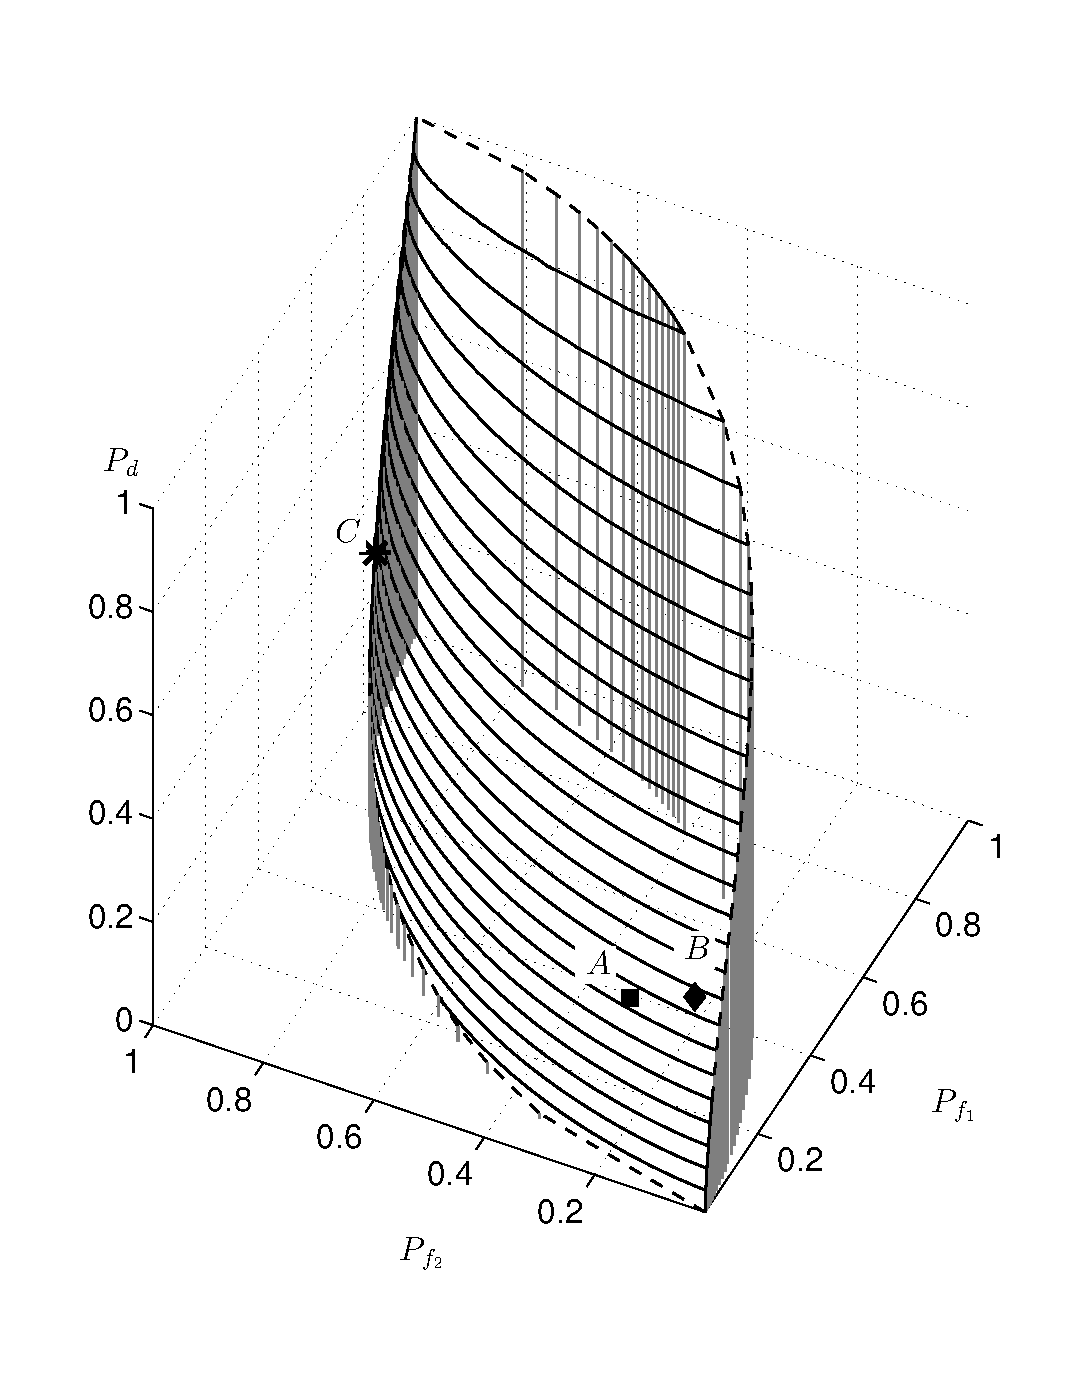
\includegraphics[width = 12cm]{2/c21.eps}
\caption{The ROC surface for $k_1$, $k_2$ range from $-30$ to $30$ with step $0.1$}
\label{fig: 2.1}
\end{figure}

It is interesting to observe that under the framework of ENP Test, for a given $(P_{f_1}, P_{f_2})$  ($P_{f_1}, P_{f_2}\in [0, 1]$) the associated $P_d$ may not exists. 
Recall in the case of binary hypotheses testing (Traditional Neyman Pearson Test), for a given $P_f \in [0, 1]$, there always exists a corresponding $P_d$. 

Now let us consider points $A$ and $B$ on the ROC surface, which are marked with $\blacksquare$ and $\diamondsuit$, respectively.  The coordinate of point $A$ is $(P_{f_1}, P_{f_2}, P_d) = (0.0841, 0.1761, 0.2868)$; and the coordinate of point $B$ is  $(P_{f_1}, P_{f_2}, P_d) = (0.0807, 0.0570, 0.3344)$. We can see even through $P_{f_1}$ and $P_{f_2}$ of point $A$ is larger than that of point $B$, the probability of detection of point $A$ is  smaller than that of point $B$.  
Unlike NP test, where $P_d$ is always non-decrease when $P_f$ increases, in the case of multiple hypotheses testing (Extended Neyman Pearson Test), $P_d$ is not always an non-decreasing function of  $P_{f_i}$ ($i=1, ..., M$).

Finally we consider point $C$ on the ROC surface, which is marked by $\ast$. The coordinate of point $C$ is $(P_{f_1}, P_{f_2}, P_d) = (0.7291, 0.9454, 0.3819)$. We can observe, in this case the value of $P_d$ is smaller than the value of $P_{f_1}$ and $P_{f_2}$, i.e. under the framework of ENP Test, $P_d \geq P_{f_i}$  ($i = 1, ..., M$) does not always hold (Qian Zhang arrives at the same conclusion in  \cite{zhang1999design, zhang2000efficient} using different method). 

\subsection{Three Lemmas of ENP Test}

Next we presents three lemmas concerning the properties of ENP test.

\noindent \textbf{Condition 1}
\textit{
\noindent Let $f_i(x) \;\;i=0, 1, ..., M$ be the PDF induced by hypothesis $H_i$, and define $g(x) = f_0(x) - \sum_{j=1}^{M} k_jf_j(x)$ where $k_i$  ($i = 1, 2, ..., M$) are real numbers. Let $\mathcal{D} \in \mathbb{R}$ be an open set such that $\int_{\bar{\mathcal{D}}}f_i(x)=0\;\;i = 1, 2, ..., M$. Furthermore,  if $x_0$ is a solution  for $g(x) = 0 \;\;(x \in \mathcal{D})$, there exists an integer $n$ such that  the $n$ order derivative of $g(x_0)$ is not equal to zero $(g^{(n)}(x_0) \neq 0)$.
}

\noindent \textbf{Lemma 1}
\noindent \textit{
Let $f_0$, $f_1$, ..., $f_M$ be PDFs defined on set $\mathcal{D}$ and $f_i(x) \neq 0$ holds a.e. on $\mathcal{D}$ ($i=0, 1,..., M$). For given constants $c_1, ..., c_M \in (0, 1)$, let $\mathcal{C}_\delta$ denote a set of decision rule,  such that for every $\delta \in \mathcal{C}_\delta$, we have $P_{f_i} \leq c_i$.
%No. 1
%\\\textnormal{(\rmnum{1})} Among all members of $\mathcal{C}_\mathcal{S}$ there exists one that maximizes $P_d$.
%No.2
\\ If  $\delta^{\ast}$ is a member of $\mathcal{C}_\delta$ and it maximize $P_d$ among all members of $\mathcal{C}_\delta$, then there exists non-negative constants $k_1, ..., k_M$ such that $\delta^\ast$ can be written in form of  
\begin{equation}
f_0(x) \substack{H_0 \\ \geq \\ < \\ \bar{H}_0} \sum_{j=1}^{M}k_jf_j(x)
\end{equation}
Moreover, under decision rule $\delta^\ast$ if $P_{f_i} $ is strictly  below the constraint $c_i$, i.e. $P_{f_i} < c_i$, the associated $k_i = 0$. 
}

Qian Zhang arrives at the same conclusion in \cite{zhang1999design, zhang2000efficient} through analysing the performance of $P_d$ with respect to $k_i$. In the following we will prove \textbf{Lemma 1} using a mathematical method, in \cite{LehmannTest, dantzig1951fundamental} a similar approach is used to proved ENP Lemma (\rmnum{4}).

\noindent\textbf{PROOF}
\newcommand{\bmu}{\boldsymbol{\mu}}
Before we proceed, we will define some notations for presentation.
Define $\mathbf{c}^T = [c_1, c_2, ..., c_M]$, $\boldsymbol{\mu}_0^T = [\mu_1, ..., \mu_M]$, $\mathbf{k}^T = [k_1, k_2, ..., k_M]$ and  $\mathbf{P}_f^T = [P_{f_1}, P_{f_2}, ..., P_{f_M}]$, obviously $\mathbf{c}$, $\bmu_0$, $\mathbf{k}$ and $\mathbf{P}_f$ are vectors in $M$ dimensional Euclidean  space. Let $\bmu^T = [\bmu_0, \mu_{M+1}]$ denote a vector in $M+1$ dimensional Euclidean space. 
Let $F(\boldsymbol{\mu}_0)$ denote the largest $P_d$ under the constraints $P_{f_i} = \mu_i\;\;i = 1, ..., M$, i.e.
\begin{equation}
\label{def: F}
\begin{split}
\max&\;\;\;\;P_d = F(\bmu_0)\\
\text{s.t.}&\;\;\;\;\mathbf{P}_f = \bmu_0
\end{split}
\end{equation}
Let $G(\boldsymbol{\mu}_0)$ denote the largest $P_d$ under the constraints $P_{f_i} \leq \mu_i\;\;i = 1, ..., M$, i.e.
\begin{equation}
\label{def: G}
\begin{split}
\max&\;\;\;\;P_d = G(\bmu_0)\\
\text{s.t.}&\;\;\;\;\mathbf{P}_f \leq \bmu_0
\end{split}
\end{equation}
By comparing \eqref{def: F} and \eqref{def: G}, we can see $G(\bmu_0 \geq F(\bmu_0))$, this is because the limitation of \eqref{def: G} is looser than that in \eqref{def: F}. 
Let $P_d(\delta)$, $P_{f_i}(\delta)$ denote the $P_d$ and $P_{f_i}$ achieved by using decision rule $\delta$.
By $\mathbf{A} \leq \mathbf{B}$, $\mathbf{A} = \mathbf{B}$ and  $\mathbf{A} \geq \mathbf{B}$ we mean that every element of $\mathbf{A}$ is no larger than, equal to and no smaller than its corresponding element of $\mathbf{B}$, respectively. 
By $\mathbf{A} \neq 0$, we mean that every element of $\mathbf{A}$ is not equal to $0$. 
Let $G'$ denote the hyper surface achieved by $G(\bmu_0) = \mu_{M+1}$, where $\bmu_0 \in [0, 1]$, i.e.
\begin{equation}
\label{def: G'}
\{(\bmu_0, \mu_{M+1}) \in G' | \bmu_0 \in [0, 1] \;\;\text{and}\;\;\mu_{M+1} = G(\bmu_0) \}
\end{equation}
Let $G_s$ denote the set of points in $M+1$ Euclidean space such that 
\[
 \{(\boldsymbol{\mu}_0, \mu_{M+1})\in G_s | \boldsymbol{\mu}_0\in [0, 1]\;\; \text{and }\;\;\mu_{M+1} \in [0, G(\mathbf{\bmu_0})]
    \}
\]
we can see $G_s$ is a space enclosed by $G'$, $\mu_i = 1$ and $\mu_{M+1}=0$ ($i=1, ..., M$).
Let $\mathcal{N}$ represents the set of points in $M+1$ dimensional Euclidean space such that  
\begin{equation}
\begin{split}
\{(\mu_1, \mu_2, ..., \mu_{M+1})\in \mathcal{N} &| \mu_i = \int_{\mathcal{S}}f_i(x)\mathrm{d}x \;\;i=1, ..., M,\\
                                            &  \mu_{M+1}=\int_{\mathcal{S}}f_{M+1}(x)\mathrm{d}x \;\;\text{ for any subset $\mathcal{S}$ of $\mathcal{D}$}\}
\end{split}
\end{equation}
we can see, $\mathcal{N}$ is the set of $(\bmu_0, \mu_{M+1})=(\mathbf{P}_f(\delta), P_d(\delta))$, where $\delta$ could be any possible decision rule. Moreover, from the definition of $\mathcal{N}$ and $F(\bmu_0)$ we can conclude if $(\bmu_0, \mu_{M+1}) \in \mathcal{N}$, we have $\mu_{M+1} \leq F(\bmu_0)$. 
To see it, assume $\mu_{M+1} > F(\bmu_0)$. Then there is a decision rule $\delta$ such that $P_{f_i}(\delta) = \mu_i$ ($i=1, ..., M$) and $P_d(\delta) > F(\bmu_0)$. This is contradictory with the definition of $F(\bmu_0)$. Hence we can conclude $\mu_{M+1} \leq F(\bmu_0)$.

The whole proof will be divided into following parts: first we will first prove $G(\boldsymbol{\mu}_0)$ is a convex, non-decreasing function and when $\boldsymbol{\mu}_0 \neq 0$, $G(\boldsymbol{\mu}_0) > 0$;
secondly it will be shown that $G_s$ is a convex set and $\mathcal{N} \subseteq G_s$; 
after that we will illustrate for any points $(\mu_1^0, \mu_2^0, ..., \mu_{M+1}^0) \in G'$, there exists a non-negative $\mathbf{k}$ such that for any $(\mu_1, \mu_2, ..., \mu_{M+1}) \in G_s$, $\mu_{M+1} - \sum_{i=1}^{M}k_i\mu_i \leq \mu_{M+1}^0 - \sum_{i=1}^{M}k_i\mu_i^0$ holds;  
in the end, we will prove for any $\mathbf{c}$, there exists non-negative $\mathbf{k}$ such that the optimal decision rule to achieve the largest $P_d$ under constraint $\mathbf{P}_f \leq \bmu_0$ can be written in form of 
\[
\delta^\ast:\;\;\;\;f_0(x) \substack{H_0 \\ > \\ < \\ \bar{H}_0} \sum_{i=1}^{M}k_if_i(x)\,.
\]

Firstly we will prove $G(\bmu_0)$ is a convex non-decreasing function for $\bmu_0 \in [0, 1]$.
 Let $\boldsymbol{\mu}^1$ and  $\boldsymbol{\mu}^2$ be two points on $G'$ with coordinates $(\boldsymbol{\mu}^1_0, \mu_{M+1}^1)$ and $(\boldsymbol{\mu}^2_0, \mu_{M+1}^2)$, i.e. $\mu_{M+1}^1 = G(\boldsymbol{\mu}_0^1)$ and $\mu_{M+1}^2 = G(\boldsymbol{\mu}_0^2)$. Let $\delta_1$ be the decision rule which can achieved the largest $P_d$ under the constraint $\mathbf{P}_f \leq \boldsymbol{\mu}_0^1$ and $\delta_2$ be the decision rule which can achieved the largest $P_d$ under the constraint $\mathbf{P}_{f} \leq \boldsymbol{\mu}_0^2$. So we can see $\mu_{M+1}^1 = P_d(\delta^1) = G(\boldsymbol{\mu}_0^1)$, $\mu_{M+1}^2 = P_d(\delta^2)=G(\boldsymbol{\mu}_0^1)$, $P_f(\delta^1) \leq \boldsymbol{\mu}^1_0$ and $P_f(\delta^2) \leq \boldsymbol{\mu}^2_0$.

Construct a new randomized new test $\delta^3$, where $\delta^1$ and $\delta^2$ are used with equal probability. With decision rule $\delta^3$, we have $P_d(\delta^3) = 0.5P_d(\delta^1)+0.5P_d(\delta^2) = 0.5G(\bmu_0^1) + 0.5G(\bmu_0^2)$ and $\mathbf{P}_{f}(\delta^3) = 0.5\mathbf{P}_f(\delta^1)+0.5\mathbf{P}_f(\delta^2) \leq 0.5\boldsymbol{\mu}^1_0 + 0.5\boldsymbol{\mu}^2_0 $. Let $\delta'$ denote the optimal decision rule for 
 \begin{equation}
 \begin{split}
 \max&\;\;\;\;P_d\\
 \text{s.t.}&\;\;\;\;\mathbf{P}_f \leq 0.5\boldsymbol{\mu}^1_0 + 0.5\boldsymbol{\mu}^2_0
 \end{split}
 \end{equation}
then obviously $P_d(\delta') \geq P_d(\delta^3)$ (otherwise $\delta'$ cannot be the optimal decision rule), i.e. $G(0.5\boldsymbol{\mu}^1_0 + 0.5\boldsymbol{\mu}^2_0) > P_d(\delta^3)$. Since $P_d(\delta^3) = 0.5 G(\boldsymbol{\mu}^1_0)+ 0.5 G(\boldsymbol{\mu}^2_0)$, the equation can be written as 
\begin{equation}
G(0.5\boldsymbol{\mu}^1_0 + 0.5\boldsymbol{\mu}^2_0) \geq 0.5 G(\boldsymbol{\mu}^1_0)+ 0.5 G(\boldsymbol{\mu}^2_0)
\end{equation}
Hence $G(\bmu_0)$ is a convex function for $\bmu_0 \in [0, 1]$.

According to the definition of $G(\bmu_0)$, when $\mu_i$ increases, the value of $G(\bmu_0)$ will not decrease, we can conclude $G(\bmu_0)$ is also a non-decreasing function of $\bmu_0$. 

Next we will show when $\boldsymbol{\mu}_0 \neq 0$, $G(\boldsymbol{\mu}_0) > 0$.

Let $\delta^\ast$ be the optimal decision rule for $\bmu_0$, by optimal decision rule we mean this decision rule can get the largest $P_d$ under the constraint $\mathbf{P}_f \leq \bmu_0$. According to \cite{zhang2000efficient}, there exists at least one $P_{f_i}(\delta^\ast) = \mu_i$ ($i=1, ..., M$). Without losing generality, let $P_{f_l}(\delta^\ast) = \mu_l$, i.e. $\int_{\mathcal{S}^\ast}f_l(x)\mathrm{d}x = \mu_l \neq 0$. Hence we can conclude the measurement of $\mathcal{S}^\ast$  is not zero. Since we know $f_0(x) \neq 0$ a.e. on $\mathcal{D}$, we can conclude $\int_{\mathcal{S}^\ast}f_0(x)\mathrm{d}x > 0$, i.e. $G(\bmu_0) > 0$. 

In the following, we will consider the property of $G_s$. First we will prove $G_s$ is a convex set. 

Let $\boldsymbol{\mu}^1$ and  $\boldsymbol{\mu}^2$ be two points in $G_s$ with coordinates $(\boldsymbol{\mu}^1_0, \mu_{M+1}^1)$ and $(\boldsymbol{\mu}^2_0, \mu_{M+1}^2)$. According to the definition of $G_s$, we have $0 \leq \bmu_0^1 \leq 1$, $0 \leq \boldsymbol{\mu}^2_0 \leq 1$, $0 \leq \mu_{M+1}^1 \leq G(\boldsymbol{\mu}_0^1)$ and  $0 \leq \mu_{M+1}^2 \leq G(\boldsymbol{\mu}_0^2)$.

Let $\boldsymbol{\mu}^3$ be the middle point between $\boldsymbol{\mu}^1$ and $\boldsymbol{\mu}^2$ with coordinate $(\bmu_0^3, \mu_{M+1}^3)$, where  $ \bmu_0^3 = 0.5\boldsymbol{\mu}_0^1 + 0.5 \boldsymbol{\mu}_0^2$ and $\mu_{M+1}^3 = 0.5 \mu_{M+1}^1 + 0.5 \mu_{M+1}^2$. Next we will show $\bmu^3 \in G_s$.  

Since $\bmu^1_0, \bmu^2_0 \in [0, 1]$, we can conclude $\bmu_0^3 = 0.5 \bmu^1_0+ 0.5\bmu^2_0 \in [0, 1]$. Since $0 \leq \mu_{M+1}^1 \leq G(\boldsymbol{\mu}_0^1)$,  $0 \leq \mu_{M+1}^2 \leq G(\boldsymbol{\mu}_0^2)$, we can conclude 
\[
0 \leq \mu_{M+1}^3 = 0.5\mu_{M+1}^1 + 0.5\mu_{M+1}^2 \leq 0.5 G(\bmu_0^1) + 0.5G(\bmu_0^2) \leq G(0.5 \bmu_0^1+0.5\bmu_0^2) = G(\bmu^3_0)\,.
\]
$0.5 G(\bmu_0^1) + 0.5G(\bmu_0^2) \leq G(0.5 \bmu_0^1+0.5\bmu_0^2)$ comes form the fact that $G(\bmu_0)$  is a convex function. Since we have proved $\bmu^3_0 \in [0, 1]$ and $\mu_{M+1}^3 \in [0, G(\bmu^3_0)]$, we can see $\bmu^3 \in G_s$, i.e. $G_s$  is a convex set.  

Next we will prove $\mathcal{N} \subseteq G_s$, i.e. $\forall (\mu_0, ..., \mu_{M+1}) \in \mathcal{N}$, this point also belongs to set $G_s$.
In previous we have proved, $\forall (\mu_1^0, ..., \mu_{M+1}^0) \in \mathcal{N}$, we have $\mu_i^0 \in [0, 1]$ ($i = 1, ..., M$) and $\mu_{M+1}^0 \in [0, F(\bmu_0^0)]$, where $\bmu_0^0 = [\mu_1^0, ..., \mu_M^0]$. Since   $G(\bmu_0^0) \geq F(\bmu_0^0)$, we can see $\mu_{M+1}^0 \in [0, G(\bmu_0^0)]$, i.e.  $(\mu_1^0, \mu_2^0, ...., \mu_{M+1}^0) \in G_s$ and  $\mathcal{N} \subseteq G_s$.

In the following we will prove for any points $(\mu_1^0, \mu_2^0, ..., \mu_{M+1}^0)$ belong to $G'$, there exists non-negative $\mathbf{k}$ such that for any $(\mu_1, \mu_2, ..., \mu_{M+1}) \in G_s$, $\mu_{M+1} - \sum_{i=1}^{M}k_i\mu_i \leq \mu_{M+1}^0 - \sum_{i=1}^{M}k_i\mu_i^0$ holds. A similar proof is given in \cite{LehmannTest, dantzig1951fundamental}.

Assume $(\mu_0^0, \mu_1^0, ..., \mu_{M+1}^0)$ is a point on the $G'$ surface, i.e. $\mu_{M+1}^0 = G(\bmu_0^0)$, where $\bmu_0^0 = [\mu_0^0, \mu_1^0, ..., \mu_{M}^0]$. According to the definition of $G_s$, for any positive $\epsilon$, point $(\mu_0^0, \mu_1^0, ..., \mu_{M+1}^0+\epsilon) \notin G_s$. Hence we can conclude $(\mu_1^0, ..., \mu_{M+1}^0)$ is a boundary point of $G_s$.  
Since $G_s$ is a convex set and $(\mu_0^0, \mu_1^0, ..., \mu_{M+1}^0)$ is a boundary point of $G_s$,  
there exists an $M+1$-dimensional hyperplane $\Pi$ through this point such that $\Pi$ contains only boundary points of $G_s$ and $G_s$ lies entirely on one sides of $\Pi$  \cite{dantzig1951fundamental}. 
 There exists $k_i^0$ ($i=1, ..., M+1$) such that the expression of $\Pi$ can be written as
\begin{equation}
\label{PI}
k_{M+1}^0\mu_{M+1} - \sum_{i=1}^{M}k_i^0\mu_i = k_{M+1}^0\mu_{M+1}^0 - \sum_{i=0}^{M}k_i^0\mu_i^0
\end{equation}

In previous part we have proved when $\mu^0_i\neq 0$ ($i=1, ..., M$), $\mu_{M+1}^0 > 0$, i.e. there exists a $\mu_{M+1}' = \frac{\mu_{M+1}^0}{2}$ such that $\mu_{M+1}' \in (0, \mu_{M+1}^0)$. From the definition of $G_s$, it is easy to know $(\mu^0_1, ..., \mu^0_M, \mu_{M+1}')$ also belongs to set $G_s$. Besides that, since $\mu^0_i \in (0, 1)$ ($i=1, ..., M$) and $\mu_{M+1}' \in (0, \mu_{M+1}^0)$, we can see $(\mu_1^0, \mu_2^0, ..., \mu_{M+1}')$ is an inner point of $G_s$, i.e. point $(\mu^0_1, ..., \mu^0_M, \mu_{M+1}')$ is not contained by hyperplane $\Pi$. We can conclude 
\[
k_{M+1}^0\mu_{M+1}' - \sum_{i=1}^{M}k_i^0\mu_i^0 \neq k_{M+1}^0\mu_{M+1}^0 - \sum_{i=0}^{M}k_i^0\mu_i^0
\]
\[
\therefore k_{M+1}^0\mu_{M+1}' \neq k_{M+1}^0\mu_{M+1}^0
\]
\[
\therefore k_{M+1}^0 \neq 0
\]
 $\Pi$ can be written as
\begin{equation}
\label{PI2}
\mu_{M+1} - \sum_{i=1}^{M}k_i\mu_i = \mu_{M+1}^0 - \sum_{i=0}^{M}k_i\mu_i^0
\end{equation}
where $k_i = \frac{k_i^0}{k_{M+1}}$. 

Since  $G_s$ lies entirely on one side of \eqref{PI2}, and since when $(\mu_1, ... ,\mu_M, \mu_{M+1})=(\mu_1^0, ..., \mu_M^0, 0)$, the left hand member of \eqref{PI2} is smaller than the right hand member, hence we can conclude 
\begin{equation}
\mu_{M+1} - \sum_{i=1}^{M}k_i\mu_i \leq \mu_{M+1}^0 - \sum_{i=0}^{M}k_i\mu_i^0
\label{PI3}
\end{equation}
holds for all points belong to $G_s$ \cite{dantzig1951fundamental}. 

Up to now, we have proved $ \forall (\bmu_0^0, \mu_{M+1}^0) \in G'$, there exists constants $k_1$, ..., $k_M$ such that
\begin{equation}
\mu_{M+1} - \sum_{i=1}^{M}k_i\mu_i \leq \mu_{M+1}^0 - \sum_{i=0}^{M}k_i\mu_i^0
\label{PPI3}
\end{equation}
holds for all points belong to $G_s$. In the following, we will illustrate in order to satisfy condition \eqref{PPI3}, the constants $k_i$ must be non-negative.   

Now consider another point on the $G'$ with coordinate $(\mu_1^0, ..., \mu_l^0+\epsilon, ..., \mu_M^0, \mu_{M+1}')$, where $\epsilon > 0$. Since $\mu_l^0 \in (0, 1)$, there always exists a positive $\epsilon$ satisfying $\mu_l^0 + \epsilon \in (0, 1]$. Since both points $(\mu_1^0, ..., \mu_l^0, ..., \mu_M^0, \mu_{M+1}^0)$ and $(\mu_1^0, ..., \mu_l^0+\epsilon, ..., \mu_M^0, \mu_{M+1}')$ lies on $G'$, we can conclude $G([\mu_1^0, ..., \mu_l^0, ...., \mu_M^0]) = \mu_{M+1}^0$ and $G([\mu_1^0, ..., \mu_l^0 + \epsilon, ...., \mu_M^0]) = \mu_{M+1}'$. As we have proved $G(\bmu_0)$ is a non-decreasing function, it is easy to see $\mu_{M+1}' \geq \mu_{M+1}^0$.

Substitute point $(\mu_1^0, ..., \mu_i^0+\epsilon, ..., \mu_M^0, \mu_{M+1}')$  into equation \eqref{PI3}, we have
\begin{equation}
\mu_{M+1} - k_1\mu_1^0 - ... - k_l(\mu_l^0+\epsilon)- ... - k_M\mu_M^0 \leq \mu_{M+1} - k_1\mu_1^0 - ... - k_l\mu_l^0- ... - k_M\mu_M^0
\end{equation}
\begin{equation}
\therefore \mu_{M+1}' - k_l(\mu_l^0+\epsilon)\leq \mu_{M+1}^0 - k_l\mu_l^0
\end{equation}
\begin{equation}
\mu_{M+1}' - \mu_{M+1}^0 \leq k_l\epsilon
\end{equation}
\[
\therefore k_l \geq \frac{\mu_{M+1}' - \mu_{M+1}^0}{\epsilon} \geq 0
\]
Hence we can conclude for any point $(\mu_1^0, \mu_2^0, ..., \mu_{M+1}^0)$ belongs to $G_s$, there exists a non-negative $\mathbf{k}$ such that 
\begin{equation}
\mu_{M+1} - \sum_{i=1}^{M}k_i\mu_i \leq \mu_{M+1}^0 - \sum_{i=1}^{M}k_i\mu_i^0
\end{equation}
holds for any $(\mu_1, \mu_2, ..., \mu_{M+1}) \in G_s$.

For the given constants $\mathbf{c}$ ($\mathbf{c} \in (0, 1)$), 
 assume decision rule $\delta^\ast$  achieves the largest $P_d$  under the constraint $\mathbf{P}_f \leq \mathbf{c}$. In the following we will prove there exists non-negative $\mathbf{k}$  such that $\delta^\ast$ can be written in form of 
\[
f_0(x) \substack{H_0 \\ > \\ < \\ \bar{H}_0 } \sum_{i=1}^{M}k_if_i(x)\,.
\]

According to the definition of $G(\bmu_0)$, we can see $P_d(\delta^\ast) = G(\mathbf{c})$. Since $(\mathbf{c}, G(\mathbf{c}))$is a point on the hyper surface $G'$, we can see there exists non-negative $\mathbf{k}$ such that for any  $(\mu_1, ..., \mu_{M+1}) \in G_s$, following equation holds 

\begin{equation}
\label{TEMP}
\mu_{M+1} - \sum_{i=1}^{M}k_i\mu_i \leq G(\mathbf{c}) - \sum_{i=0}^{M}k_ic_i
\end{equation}
Since $P_{f_i}(\delta^\ast) \leq c_i$ (for $i=1, ..., M$) and $k_i \geq 0$, we know
\[
k_ic_i \geq k_iP_{f_i}(\delta^\ast)
\]
\[
\therefore \sum_{i=1}^{M}k_ic_i \geq \sum_{i=1}^{M}k_iP_{f_i}(\delta^\ast)
\]
Hence we have
\begin{equation}
\label{con: 1}
G(\mathbf{c}) - \sum_{i=1}^{M}k_ic_i \leq G(\mathbf{c}) - \sum_{i=1}^{M}k_iP_{f_i}(\delta^\ast)\,.
\end{equation}
Combine \eqref{TEMP} and \eqref{con: 1}, we have 
\begin{equation}
\label{equ: TEMP3}
\mu_{M+1} - \sum_{i=1}^{M}k_i\mu_i \leq G(\mathbf{c}) - \sum_{i=0}^{M}k_ic_i \leq G(\mathbf{c}) - \sum_{i=0}^{M}k_iP_{f_i}(\delta^\ast)
\end{equation}
\begin{equation}
\label{ASD}
\therefore \mu_{M+1} - \sum_{i=1}^{M}k_i\mu_i \leq G(\mathbf{c}) - \sum_{i=0}^{M}k_iP_{f_i}(\delta^\ast)
\end{equation}
Substitute $G(\mathbf{c}) = P_d(\delta^\ast)$ into \eqref{ASD}, 
\begin{equation}
\label{TEMP2}
\mu_{M+1} - \sum_{i=1}^{M}k_i\mu_i \leq P_d(\delta^\ast) - \sum_{i=0}^{M}k_iP_{f_i}(\delta^\ast)\,,
\end{equation}
where $(\mu_0, ..., \mu_{M+1}) \in G_s$.

Since $\mathcal{N} \subseteq G_s$, \eqref{TEMP2} also hold for any point belongs to $\mathcal{N}$.
According to the definition of $\mathcal{N}$, the expression of $\mu_i$  can be written as 
\begin{equation}
\label{def: mu}
\begin{cases}
\mu_i = \int_{\mathcal{S}}f_i(x)\mathrm{d}x \;\;\;\;i = 1, ..., M\\
\mu_{M+1} = \int_{\mathcal{S}}f_{0}(x)\mathrm{d}x
\end{cases}
\end{equation}
where $\mathcal{S}$ can be any subset of domain $\mathcal{D}$. 

$P_{f_i}(\delta^\ast)$ and $P_{d}(\delta^\ast)$ can be written as
\begin{equation}
\label{def: pfd}
\begin{cases}
P_{f_i}(\delta^\ast) = \int_{\mathcal{S}^\ast}f_i(x)\mathrm{d}x\;\;\;\;i=1, ..., M\\
P_d(\delta^\ast) = \int_{\mathcal{S}^\ast}f_0(x)\mathrm{d}x
\end{cases}
\end{equation}
Substitute \eqref{def: mu} and \eqref{def: pfd} into \eqref{TEMP2}, we have: 
\[
\int_{\mathcal{S}}f_{0}(x)\mathrm{d}x - \sum_{i=1}^{M}k_i\int_{\mathcal{S}}f_i(x)\mathrm{d}x \leq \int_{\mathcal{S}^\ast}f_{0}(x)\mathrm{d}x - \sum_{i=1}^{M}k_i\int_{\mathcal{S}^\ast}f_i(x)\mathrm{d}x
\]
\[
\therefore 
\int_{\mathcal{S}}f_{0}(x)\mathrm{d}x - \sum_{i=1}^{M}\int_{\mathcal{S}}k_if_i(x)\mathrm{d}x \leq \int_{\mathcal{S}^\ast}f_{0}(x)\mathrm{d}x - \sum_{i=1}^{M}\int_{\mathcal{S}^\ast}k_if_i(x)\mathrm{d}x
\]
\begin{equation}
\label{TEMP4}
\therefore \int_{\mathcal{S}}(f_{0}(x)- \sum_{i=1}^{M}k_if_{i}(x))\mathrm{d}x \leq \int_{\mathcal{S}^\ast}(f_{0}(x)- \sum_{i=1}^{M}k_if_{i}(x))\mathrm{d}x 
\end{equation}

\eqref{TEMP4} can be fulfilled only if $\mathcal{S}^\ast$ satisfies
\[
x \in \mathcal{S}^\ast\;\;\;\;\text{if}\;\;\;\;f_{0}(x)- \sum_{i=1}^{M}k_if_{i}(x) > 0
\]
\[
x \notin \mathcal{S}^\ast\;\;\;\;\text{if}\;\;\;\;f_{0}(x)- \sum_{i=1}^{M}k_if_{i}(x) < 0
\]

Hence we can conclude for any given $\mathbf{\bmu_0} \in (0, 1)$, there exists a set of non-negative $\mathbf{k}$ such that 
the optimal decision rule can be written as 
\[
f_0(x) \substack{H_0 \\ > \\ < \\ \bar{H}_0 } \sum_{i=1}^{M}k_if_i(x)\,.
\]

Since \eqref{TEMP} holds for any point $(\mu_1, \mu_2, ..., \mu_{M+1}) \in \mathcal{N}$ and $(\mathbf{P}_f(\delta^\ast), P_d(\delta^\ast)) \in \mathcal{N}$, we can conclude 
\begin{equation}
\label{TEMP5}
P_d(\delta^\ast) - \sum_{i=0}^{M}k_iP_{f_i}(\delta^\ast) \leq G(\mathbf{c}) - \sum_{i=0}^{M}k_ic_i
\end{equation}
From \eqref{con: 1} and \eqref{TEMP5}  we can conclude
\[
P_d(\delta^\ast) - \sum_{i=0}^{M}k_iP_{f_i}(\delta^\ast) =  G(\mathbf{c}) - \sum_{i=0}^{M}k_ic_i
\]
\[
\therefore  \sum_{i=0}^{M}k_iP_{f_i}(\delta^\ast) =  \sum_{i=1}^{M}k_ic_i
\]
Since $k_iP_{f_i}(\delta^\ast) \leq k_ic_i$ (for $i=1, ..., M$), the above equation can be fulfilled only when $k_iP_{f_i} = k_ic_i$ (for $i=1, ..., M$). When $P_{f_i}(\delta^\ast)$ is strictly below $c_i$ ($P_{f_i}(\delta^\ast) < c_i$), $k_i$ must be zero.

Q.E.D.

\noindent \textbf{Lemma 2}
\textit{
\noindent Under}
\textbf{Condition 1}
\textit{, let $\mathbf{P}$ be a point with coordinate $(P_d, P_{f_1}, ..., P_{f_M})$ on the ROC surface of the EPN test. If there exists a tangent hyperplane at $\mathbf{P}$, then its normal is parallel to the vector $\mathbf{n} = (-1, k_1, ..., k_M)$, where $k_i$ are the parameters of the ENP test achieving $\mathbf{P}$.
}

\noindent\textbf{PROOF}
Define $\mathbf{k} = [k_1, k_2, ..., k_M]^T$ and $\mathbf{P}_f = [P_{f_1}, P_{f_2}, ..., P_{f_M}]^T$. Since both $P_d$ and $\mathbf{P}_f$ are functions of $\mathbf{k}$, $\mathbf{P}_f(\mathbf{k}_0)$ denotes the value of $\mathbf{P}_f$ when $\mathbf{k} = \mathbf{k}_0$ and $P_d(\mathbf{k}_0)$ denotes the value of $P_d$ when $\mathbf{k} = \mathbf{k}_0$. Using Taylor's expansion for $\mathbf{P}_f$ and $P_d$,
\begin{equation}
\label{pro: pd}
P_d = P_d(\mathbf{k}_0) + \frac{\mathrm{d}P_d}{\mathrm{d}\mathbf{k}^T}\bigg{|}_{\mathbf{k}=\mathbf{k_0}}(\mathbf{k} - \mathbf{k}_0)
+ o(\mathbf{k} - \mathbf{k}_0)
\end{equation}

\begin{equation}
\label{pro: pf}
\mathbf{P}_f = \mathbf{P}_f(\mathbf{k}_0) + \frac{\mathrm{d}\mathbf{P}_f}{\mathrm{d}\mathbf{k}^T}\bigg{|}_{\mathbf{k}=\mathbf{k_0}}(\mathbf{k} - \mathbf{k}_0)
+ o(\mathbf{k} - \mathbf{k}_0)
\end{equation}
here $\mathbf{k} \rightarrow \mathbf{k}_0$.

Consider the hyperplane $y$ as a function of $\mathbf{x}$ defined by
\begin{equation}
\label{pro: x}
\mathbf{x} = \mathbf{P}_f(\mathbf{k}_0) + \frac{\mathrm{d}\mathbf{P}_f}{\mathrm{d}\mathbf{k}^T}\bigg{|}_{\mathbf{k}=\mathbf{k_0}}(\mathbf{z} - \mathbf{k}_0)
\end{equation}
\begin{equation}
\label{pro: y}
y = P_d(\mathbf{k}_0) + \frac{\mathrm{d}P_d}{\mathrm{d}\mathbf{k}^T}\bigg{|}_{\mathbf{k}=\mathbf{k_0}}(\mathbf{z} - \mathbf{k}_0)
\end{equation}
The above equations construct a tangent hyperplane for the ROC surface at point $(P_d(\mathbf{k}_0), \mathbf{P}_f^T(\mathbf{k}_0))$. Combining both equations  we get

\begin{equation}
\label{pro : y2}
y = P_d(\mathbf{k}_0) + \frac{\mathrm{d}P_d}{\mathrm{d}\mathbf{k}^T}\bigg{|}_{\mathbf{k}=\mathbf{k_0}}(
\frac{\mathrm{d}\mathbf{P}_f}{\mathrm{d}\mathbf{k}^T}\bigg{|}_{\mathbf{k}=\mathbf{k_0}}
)^{-1} (\mathbf{x} - \mathbf{P}_f(\mathbf{k}_0))
\end{equation}
Hence the normal for point $(P_d(\mathbf{k}_0), \mathbf{P}_f^T(\mathbf{k}_0))$ on ROC surface can be written as
\begin{equation}
\label{vec: normal}
[-1, \frac{\mathrm{d}P_d}{\mathrm{d}\mathbf{k}^T}\bigg{|}_{\mathbf{k}=\mathbf{k_0}}(
\frac{\mathrm{d}\mathbf{P}_f}{\mathrm{d}\mathbf{k}^T}\bigg{|}_{\mathbf{k}=\mathbf{k_0}}
)^{-1}
].
\end{equation}

In the following, we will prove $ \frac{\mathrm{d}P_d}{\mathrm{d}\mathbf{k}^T}(
\frac{\mathrm{d}\mathbf{P}_f}{\mathrm{d}\mathbf{k}^T}
)^{-1} = \mathbf{k}^T
$, which can be written as
\begin{equation}
\label{pro: vec}
\frac{\mathrm{d}P_d}{\mathrm{d}\mathbf{k}^T} = \mathbf{k}^T \frac{\mathrm{d}\mathbf{P}_f}{\mathrm{d}\mathbf{k}^T}
\end{equation}

Previous equation can be written in component form as
\begin{equation}
\label{pro: component}
\frac{\partial P_d}{\partial k_i} - \sum_{n=1}^{M}k_n\frac{\partial P_{f_n}}{\partial k_i} = 0 \;\;\;\;(i=1, 2, ..., M).
\end{equation}
Calculating the  partial derivatives results in
\begin{equation}
\label{pro: Pf par k}
\frac{\partial P_{f_n}}{ \partial k_i} = - \int_{\mathcal{D}}\delta (f_0(x) - \sum_{j=1}^{M}k_jf_j(x))f_i(x)f_n(x) \mathrm{d}x\,,
\end{equation}
\label{pro: Pd par k}
\begin{equation}\frac{\partial P_d}{ \partial k_i} = - \int_{\mathcal{D}}\delta (f_0(x) - \sum_{j=1}^{M}k_jf_j(x))f_i(x)f_0(x) \mathrm{d}x\,,
\end{equation}
where $\delta(\bullet)$ is Dirac's delta function defined as following,

\begin{equation}
\label{pro: delta}
\delta(x) = \substack{\lim \\ \epsilon \rightarrow 0} \begin{cases}
\frac{1}{\epsilon}\;\;\;\;&\text{when} \;\;x \in (-\frac{\epsilon}{2}, \frac{\epsilon}{2})\\
0\;\;\;\;&\text{otherwise}
\end{cases} \;\;\;\;
\end{equation}

Defining $g(x) = f_0(x) - \sum_{j=1}^{M} k_jf_j(x)$, \eqref{pro: component} can be written as $\int_{\mathcal{D}}\delta(g(x))g(x)f_n(x)\mathrm{d}x = 0, n = 0, 1, ..., M$.

When $g(x) \neq 0$, we have $\delta(g(x)) = 0$ and $\delta(g(x))g(x)f_i(x) = 0$.   When  $g(x) = 0$, we can solve the equation according to the definition of $\delta(\bullet)$ and consider
\begin{equation}
\label{pro: important}
\int_{\{x|g(x)\in (-\frac{\epsilon}{2}, \frac{\epsilon}{2})\}} \frac{1}{\epsilon} g(x)f_n(x) \mathrm{d}x\;\;\;\;n=0, 1, ..., M
\end{equation}

Since when $g(x) \in (-\frac{\epsilon}{2}, \frac{\epsilon}{2})$, $|g(x)| < \frac{\epsilon}{2}$,
\begin{equation}|
\int_{\{x|g(x)\in (-\frac{\epsilon}{2}, \frac{\epsilon}{2})\}} \frac{1}{\epsilon} g(x)f_i(x) \mathrm{d}x | <
\int_{\{x|g(x)\in (-\frac{\epsilon}{2}, \frac{\epsilon}{2})\}} \frac{1}{2}f_i(x) \mathrm{d}x
\end{equation}

Assume $x_s$ is one of the zero point of $g(x)$, also assume $g^\prime(x_s)$, $g^{(2)}(x_s)$, ..., $g^{(n-1)}(x_s)$ are zero but $g^{(n)}(x_s) \neq 0$ (here $n = 1, 2, ...$). Use Taylor expansion near point $x_s$,
\begin{equation}
  \label{equ: gx taylor expansion}
  g(x) = \frac{g^{(n)}(x_s)}{n!}(x - x_s)^n + o((x - x_s)^n)\,.
\end{equation}
%define
\def \LEFT{ x_s
  -\left(\frac{n!\varepsilon}{2|g^{(n)}(x_s)|}\right)^{\frac{1}{n}}}
  \def \RIGHT{ x_s
  +\left(\frac{n!\varepsilon}{2|g^{(n)}(x_s)|}\right)^{\frac{1}{n}}}
%end define
From equation \eqref{equ: gx taylor expansion}, it can be seen when $g(x)\in (-\frac{\epsilon}{2}, \frac{\epsilon}{2})$, $x \in \left(
      \LEFT, \RIGHT
  \right)$.  Define $\bigtriangleup x = \left(\frac{n!\varepsilon}{2|g^{(n)}(x_s)|}\right)^{\frac{1}{n}}$, when $\epsilon \rightarrow 0$, $\bigtriangleup x \rightarrow 0$ and
\begin{equation}
\label{pro: scale}
g(x) \in (-\frac{\epsilon}{2}, \frac{\epsilon}{2})  \Leftrightarrow x \in (x_s -\bigtriangleup x, x_s + \bigtriangleup x)
\end{equation}
 Hence when $\epsilon \rightarrow 0$ we have
\begin{equation}
\int_{\{x|g(x)\in (-\frac{\epsilon}{2}, \frac{\epsilon}{2})\}} \frac{1}{2}f_i(x) \mathrm{d}x \rightarrow
f_i(x_s)\bigtriangleup x \rightarrow 0
\end{equation}

Using the above two conclusions for $g(x) = 0$ and $g(x) \neq 0$, we get
\begin{equation}
\int_{\mathcal{D}} \delta (g(x)) g(x)f_i(x) \mathrm{d}x = 0
\end{equation}

In this way, we prove the normal for the point \textbf{P} on the ROC is $(-1, k_1, k_2, ..., k_M)$.

Q.E.D.

\noindent \textbf{Lemma 3}
\textit{
\noindent
Under}
\textbf{Condition 1}
\textit{, let $\mathbf{P}$ be a point on the ROC surface, $\frac{\partial P_d}{\partial P_{f_i}} \bigg|_P = k_i$, where $k_i$ are the parameters of ENP test achieving $\mathbf{P}$.
}

\noindent\textbf{PROOF}
The expression of tangent hyper surface for point $(P_d^0, P_{f_1}^0, ..., P_{f_M}^0)$ on the ROC hyper surface can be written as
\begin{equation}
P_d = P_d^0 + \sum_{i=1}^{M} \frac{\partial P_d}{\partial P_{f_i}}\bigg|_{P_{f_i} = P_{f_i}^0}(P_{f_i} - P_{f_i}^0)\,.
\end{equation}
Hence the normal at this point is

 $\mathbf{n} = [-1, \frac{\partial P_d}{\partial P_{f_1}}, \frac{\partial P_d}{\partial P_{f_2}}, ..., \frac{\partial P_d}{\partial P_{f_M}}]$. Since we have proved that  the normal for this point is $\mathbf{n} = [-1, k_1, k_2, ..., k_M]$, we must have
\begin{equation}
\frac{\partial P_d}{\partial P_{f_i}}\bigg|_{P} = k_i
\end{equation}

Q.E.D.

\section{Modified Extended Neyman Pearson Testing}

%define \JUDGEMENT
\def \JUDGEMENT{u(f_0(x) - \sum_{j=1}^{M}k_j f_j(x))}

In context of spectrum sensing, following problem needs to be solved,
      \begin{equation}
      \label{equ: problemstate}
      \begin{split}
      \max\;\;\;\;\;\;&P_d\\
      \text{s.t.}\;\;\;\;\;\;&\mathbf{P}_f \leq \mathbf{c}
      \end{split}
      \end{equation}

According to ENP Lemma, this problem can be solved by an ENP test only when there are parameters $k_i \geq 0, \;\;i=1, ..., M$ such that 
\begin{equation}
\label{equ: condition for ENP}
\begin{split}
c_i = \int_{-\infty}^{\infty}u(f_0 - \sum_{j=1}^{M}k_jf_j(x))f_i(x)\mathrm{d}x \;\;i = 1, ..., M
\end{split}
\end{equation}

The case when the given $c_i\;\;i = 1, 2, ..., M$ do not satisfy \eqref{equ: condition for ENP} was not considered so far. 

Next we present the Modified Extended Neyman Pearson Test (MENP) for solving \eqref{equ: problemstate}.

Before we proceed, we will define some notations for easy presentation.
Define the set $\mathcal{A}_\mathbf{c} = \{
  \mathbf{P}_f | 0 \leq P_{f_i} \leq c_i
  \;\;i=1, 2, ..., M\}\,.
$ and set $\alpha^+ \triangleq \{\mathbf{P}_f | P_{f_i} = \int_{-\infty}^{\infty} \JUDGEMENT f_i(x) \mathrm{d}x, \text{where\;\;} k_i \geq 0 \;\;i=1, ..., M\}$.

\noindent \textbf{Modified Extended Neyman Pearson Test}
\noindent \textit{
\\\textnormal{(\rmnum{1})} Assume $\mathbf{c} \in \alpha^+$. Then there must be a $\mathbf{k}^0 = [k_1^0, k_2^0, ..., k_M^0]^T$ with $k_i \geq 0\;\;i=1, ..., M$ satisfying
}
\begin{equation}
\label{equ:Pf}
  P_{f_i}^0 = \int_{-\infty}^{\infty} u(f_0(x) - \sum_{j=1}^{M}k_j^0f_j(x))f_i(x)\mathrm{d}x = c_i \;\; (i= 1, 2, ..., M)\,.
\end{equation}
\textit{
    and the decision rule $\delta $ solving  \eqref{equ: problemstate} is:
}
\begin{equation}
\label{equ:decision rule}
\delta:\;\;\;\;\frac{f_0(x)}{\sum_{i=1}^{M}k_i^0f_i(x)} \substack{H_0 \\ \geq \\ < \\ \bar{H}_0} 1
\end{equation}
\textit{
\noindent \textnormal{(\rmnum{2})} Assuming $\mathbf{c} \notin \alpha^+$, Let $\mathcal{C} = \mathcal{A}_{\mathbf{c}} \cap \alpha^+$, and $\mathbf{a}^0 = [a_1^0, a_2^0, ..., a_M^0]^T \in \mathcal{C}$ be such that
}
\begin{equation}
\label{equ: F0}
\max_{\mathbf{a} \in \mathcal{C}}\;\;\;\;F(\mathbf{a}) = F(\mathbf{a}^0)\\
\end{equation}
\textit{
Since $\mathbf{a}^0 \in \mathcal{A}_{\mathbf{c}} \cap \alpha^+$, from \textnormal{(\rmnum{1})} we have that there exists a vector $\mathbf{k}^0$ such that \eqref{equ:decision rule}  maximizes $P_d$ under the constraints $P_{f_i} = a_i^0, \;i=1, ..., M$. Here since $a_i^0 \leq c_i^0, \;i=1, ..., M$ this decision rule  solves \eqref{equ: problemstate}.
}

Next we will show \textbf{Modified Extended Neyman Pearson Test} can provide an optimal solution for \eqref{equ: problemstate}.

\textbf{PROOF}
MENP (\rmnum{1}) is a direct conclusion from ENP Lemma, we will consider MENP (\rmnum{2}). Assume $\mathbf{a}^0$ satisfy
\begin{equation}
\label{a0}
\max_{\mathbf{a}\in\mathcal{C}} F(\mathbf{a}) = F(\mathbf{a^0})
\end{equation}
and decision rule $\delta^0$ maximizes $P_d$ under the constraints $P_{f_i} = a^0_i$ ($i = 1, ..., M$). Since $\mathbf{a}^0 \in \alpha^+$, from (\rmnum{1}) we know there exists $k_1^0, ..., k_M^0$ such that $\delta^0$ can be written in form of 
\[
\delta^0:\;\;\;\;\frac{f_0(x)}{\sum_{i=1}^{M}k_i^0f_i(x)} \substack{H_0 \\ \geq \\ < \\ \bar{H_0}} 1\,.
\] 
From the definition of $F(\mathbf{a})$, we know $F(\mathbf{a_0}) = P_d(\delta^0)$.

In the following, we  will prove $\delta^0$ is the optimal solution for \eqref{equ: problemstate}. 
Assume  $\delta^0$ does not achieve the largest $P_d$ under constraints $P_{f_i} \leq c_i$ ($i=1, ..., M$) and let $\delta'$ be the optimal decision rule for \eqref{equ: problemstate}, hence  we can conclude
\begin{equation}
\label{condition 1}
P_{f_i}(\delta') \leq c_i\;\;\;\;i=1, 2, ..., M\\
\end{equation}

\begin{equation}
\label{condition 2}
P_{d}(\delta') > P_d(\delta^0)
\end{equation}
From \textbf{Lemma 1}, there exists non-negative constants $k_1', ..., k_M'$ such that $\delta'$ can be written in form of 
\begin{equation}
f_0(x) \substack{H_0 \\ \geq \\ < \\ \bar{H_0}} \sum_{i=1}^{M}k_i'f_i(x)\,.
\end{equation}

The expression of $P_d(\delta')$ and $P_{f_i}(\delta')$ can be written as
\begin{equation}
\begin{cases}
\label{TEMP10}
P_{d}(\delta') &= \int_{-\infty}^{\infty} u(f_0(x) - \sum_{i=1}^{M}k_i'f_i(x)) f_0(x) \mathrm{d}x\\
P_{f_i}(\delta') &= \int_{-\infty}^{\infty} u(f_0(x) - \sum_{i=1}^{M}k_i'f_i(x)) f_i(x) \mathrm{d}x
\end{cases}
\end{equation}
where $k_i' \geq 0$.

From \eqref{condition 1} and \eqref{TEMP10}, we can conclude 
 $\mathbf{P}_f(\delta') \in \mathcal{A}_\mathbf{c} \cap \alpha^+$. Let $\mathbf{a}' = \mathbf{P}_f(\delta')$, since $\delta'$ is an ENP decision rule and it satisfies 
\begin{equation}
\mathbf{P}_f(\delta') = \mathbf{a'}\,,
\end{equation}
according to ENP Lemma (\rmnum{2}), we can see $\delta'$ achieve the largest $P_d$ under the constraint $\mathbf{P}_f = \mathbf{a'}$, i.e. 
$F(\mathbf{a}') = P_d{\delta'}$.

Since $P_d(\delta') > P_d(\delta^0)$, we have $F(\mathbf{a'}) > F(\mathbf{a^0})$. This is contradictory with the condition that $\mathbf{a^0}$ satisfy \eqref{a0}.

Hence we conclude $\delta^0$ is the optimal solution for \eqref{equ: problemstate}. $\blacksquare$

Next we present a method of finding $\mathbf{a}^0$. For a specific $\mathbf{c}$, in order to get $\mathbf{a}^0$, we need to determine the set of $\alpha^+$. We can conduct an exhaustive search over a grid of $k_1, ..., k_M$ ($k_i \geq 0$) depending on preferable accuracy and store these results ($P_d, \mathbf{P}_f, \mathbf{k}$) into a lookup table $T_1$. After that, we iterate every item in $T_1$ and put the item into table $T_2$ if the item satisfies:  $\mathbf{P}_f \leq \mathbf{c}$.
At last, we iterate every item in $T_2$ and get the largest $P_d$ and its decision rule $\mathbf{k}$.


\section{Determine the decision rule under MENP Framework}
In context of spectrum sensing, the lookup table $T_1$ can be pre-computed and stored in the detector before the detector is deployed. Once $c_i$ is changed, the detector utilizes $T_1$ to get the MENP decision  rule parameters accordingly. The size of $T_1$ depends on the value of $M$, the range and the step of $k_i$.  Assume the value of $k_i$ ranges from $0$ to $\Gamma$ with step $\tau_0$, since $T_1$ is an exhaustive lookup table on the grid of $k_1, ..., k_M$, it has $(\frac{\Gamma}{\tau_0})^M$ items. Since a linear increase of $M$ leads to an exponential increase in the size of $T_1$, the exhaustive search methods is no plausible for for the situation where $M$ is large. 

In \cite{zhang1999design, zhang2000efficient} Qian proposed an algorithm to solve this issue.  The algorithm can iteratively refine $k_i$ ($i=1, ..., M$) and generates an ENP test  such that among all ENP test with non-negative parameters it achieves the largest $P_d$ while keeping $P_{f_i}$ below the prescribed constraints. In \textbf{Lemma 1}, it has been proved that optimal decision rule for \eqref{equ: problemstate} is an ENP decision rule with non-negative $k_i$. 
We can see if a decision rule $\delta$ is an ENP test such that among all ENP test with non-negative parameters it maximize $P_d$ while keeping $\mathbf{P}_f \leq \mathbf{c}$, then $\delta$ is the optimal decision rule for \eqref{equ: problemstate}.
From the above discussion, it is clear that the decision rule generated by \cite{zhang1999design, zhang2000efficient} is the optimal decision rule for \eqref{equ: problemstate}.

The algorithm is summarized as follows. Let $t = \sum_{i=1}^{M}k_i$ and $\omega_i = \frac{k_i}{t}$. In the algorithm, $\bom$ is termed the weight of the decision rule and $t$ is termed the threshold of the decision rule. In the algorithm, only non-negative $k_i$ are considered, hence both $\omega_i, t$ are not negative. The ENP test can be written in form of 
\begin{equation}
\label{qian dec}
f_0(x) \substack{H_0 \\ \geq \\ < \\ \bar{H}_0} t\sum_{i=1}^{M}\omega_if_i(x)\,.
\end{equation}

Let $P_d$ and $\mathbf{P}_f$ denote the probability of detection and probability of false alarm of decision rule \eqref{qian dec} respectively. 
\cite{zhang2000efficient} illustrates that with $\omega_i$ ($i=1, 2, ..., M$) fixed, the probability of detection ($P_d$) and probability of false alarm ($\mathbf{P}_f$) under decision rule \eqref{qian dec} are non-increasing function with respect to $t$. 
Moreover, when the $t$ decreases from infinity to $0$, $P_d$ and $P_{f_i}$ increase from $0$ to $1$.

The algorithm contains four steps: (\rmnum{1}) initialization; (\rmnum{2}) weight adjustment; (\rmnum{3}) threshold adjustment; (\rmnum{4}) tolerance checking.

In initialization, $\omega_i$ ($i=1, 2, ..., M$)  is assigned arbitrary values on condition that $\sum_{i=1}^{M}\omega_i = 1$.  After that, the algorithm iteratively decreases the value of  $t$ from infinity to increase $P_d$ until one of probability of false alarm is equal to its constraint. In this way, the initial value of threshold is acquired. 

After that, the algorithm will begin the weights adjustment process. 
Assume before the adjustment the weight is $\bom_0$, the threshold is $t_0$ and the associated probability of detection is $P_d^0$.
In this step, with the probability of detection fixed, the algorithm modifies the value of $\bom$ and $t$ until $\mathbf{P}_f$ is strictly below $ \mathbf{c}$, i.e. using the modified decision rule, we have $\mathbf{P}_f < \mathbf{c}$ and $P_d = P_d^0$. 
Let $\delta\bom$ denote the perturbations of $\bom$ and let $\bom'$ denote the modified weight, i.e. $\bom' = \bom + \delta\bom$.  It is shown in \cite{zhang2000efficient} that in order to make $\mathbf{P}_f < \mathbf{c}$ while keeping $P_d$ unchanged, $\bom'$ should ensure $\theta(\mathbf{P}_f, \mathbf{c})$ decrease ($\theta(\mathbf{A}, \mathbf{B})$ denotes the angle between vectors $\mathbf{A}$ and $\mathbf{B}$). To do this, \cite{zhang2000efficient} proved that the direction of $\delta\bom$ must be the same as
\begin{equation}
\label{direction}
\mathbf{D} - m_\mathbf{D}\bom
\end{equation}
where 
\[
\mathbf{D} = \mathbf{P}_f - \mathbf{c}\frac{|\mathbf{P}_f|^2}{\mathbf{c}\mathbf{P}_f}
\]
and $m_{\mathbf{D}}$ represents the arithmetic sum of the elements of $\mathbf{D}$. And $\delta\bom$ can be written as
\[
\delta\bom = \lambda( \mathbf{D} - m_\mathbf{D}\bom) 
\]
here $\lambda$ is a value associated with the magnitude of $\delta\bom$.
According to \cite{zhang2000efficient}, a too large $\lambda$ may results $\theta(\mathbf{P}_f, \mathbf{c})$ increase, which is a undesirable case, while a too small value can not decrease $\theta(\mathbf{P}_f, \mathbf{c})$ very much. The algorithm chooses the value of $\lambda$ by trial and error. To do this, the algorithm choose the arithmetic average of $\mathbf{P}_f$ as the initial value of $\lambda$ and compute the new weights $\bom'$ through \eqref{direction}. 
If any element of $\bom'$ is negative, e.g. $\omega_i < 0$, the negative element will be changed to zero. This is because a negative  $\omega_i$ is not considered in this method.  
Then the algorithm use $\bom'$ to find the $t'$ such that under the new decision rule the probability of detection is equal to  $P_d^0$. To do this, with $\bom'$ fixed, the algorithm will iteratively decrease the value of $t'$ from a very large value until $P_d = P_d^0$ is satisfied. Under the new decision rule, if $\mathbf{P}_f$ is strictly below $\mathbf{c}$, the weight adjustment is finished and the algorithm will process threshold adjustment; otherwise, the algorithm reduces the value of $\lambda$ and recompute $\bom'$ and $t'$ until $\mathbf{P}_f < \mathbf{c}$  is satisfied. 

After that, the algorithm performs the threshold adjustment process. Since all probability of false alarm is strictly below its associated constraint, by revising the threshold, the probability of detection can be further improved. In this process, with $\omega_i$ ($i=1, 2, ..., M$) fixed, the algorithm iteratively decreases the value of $t$ to increase the value of $P_d$ until one of $P_{f_i}$ is equal to $c_i$.

The last step is tolerance checking. \cite{zhang2000efficient} shows that the theoretical solution satisfies a false alarm probability constraint with equality if the associated weight is non-zero; a false alarm is strictly below the constraint if the associated weight is zero. Hence in the tolerance check, the algorithm checks whether every $c_i - P_{f_i}$  is within a prescribed tolerance value if the associated $\omega_i$ is not zero. If so, it means the decision rule is closed enough to the theoretical solution and the algorithm will output the threshold and weight, if not the algorithm will start a new cycle of weight adjustment - weight adjustment - threshold adjustment - tolerance checking process process. 


\section{Relationship to Bayesian Hypotheses Testing}

